\documentclass[10pt,a4paper]{scrartcl}
\usepackage[utf8]{inputenc}
\usepackage{amsmath}
\usepackage{amsfonts}
\usepackage{amssymb}
\usepackage{graphicx}

\usepackage[bottom = 1in, left = 0.5in, right = 0.5in, top = 1in]{geometry}

\usepackage[english]{babel}
\usepackage[autostyle]{csquotes}
\usepackage{mathptmx}

\usepackage[labelfont=bf]{caption}

\usepackage[default, scale=0.95]{opensans} %% Alternatively
%% use the option 'defaultsans' instead of 'default' to replace the
%% sans serif font only.
\usepackage[T1]{fontenc}

\title{My neat title here}
\subtitle{Figures}
\date{}

\begin{document}
\maketitle

\begin{figure}[h]
	\centering
	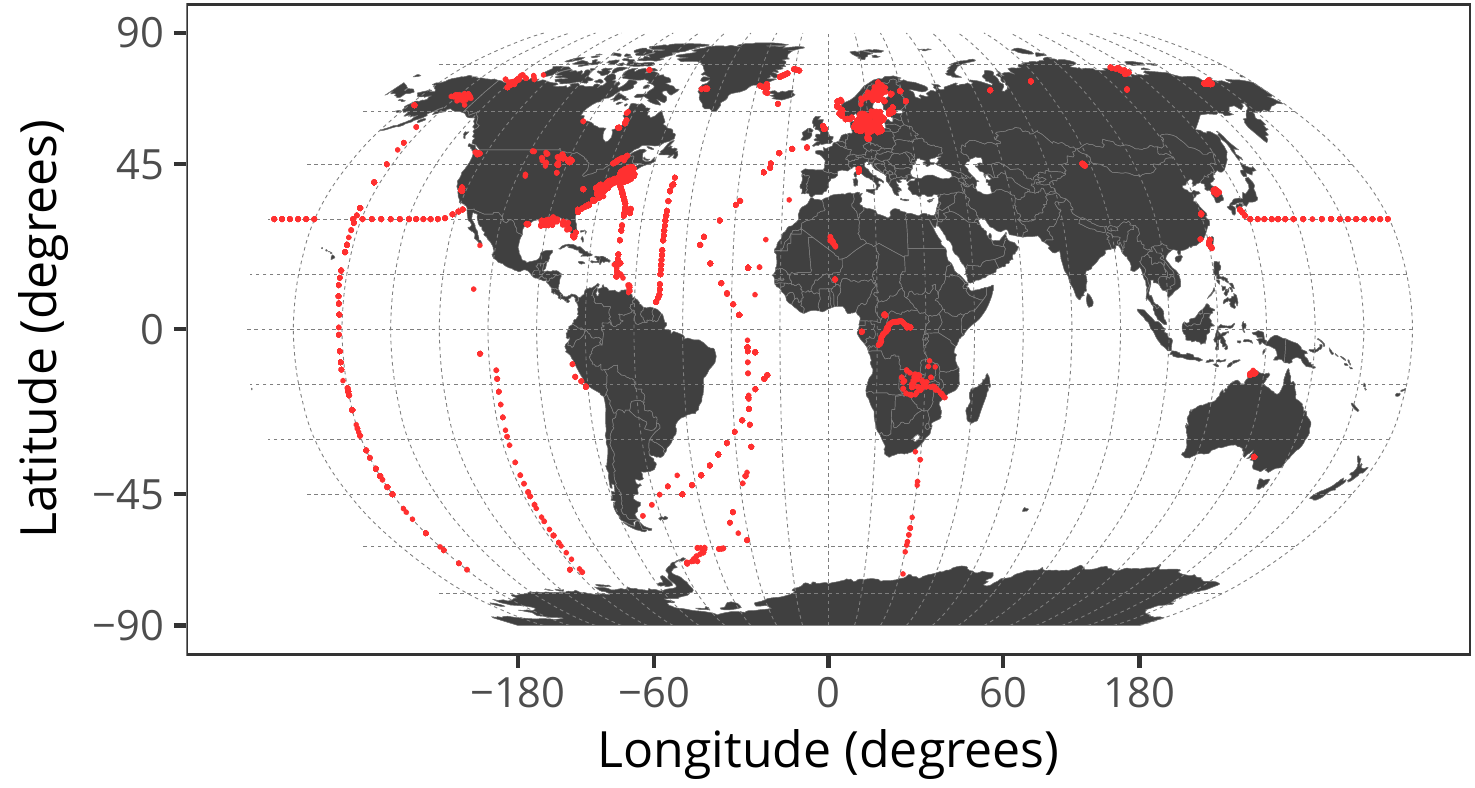
\includegraphics[scale = 1]{../../graphs/fig1}
	\caption{World map showing the spatial distribution of the study sites.}
\end{figure}

\clearpage
\newpage

\begin{figure}[h]
	\centering
	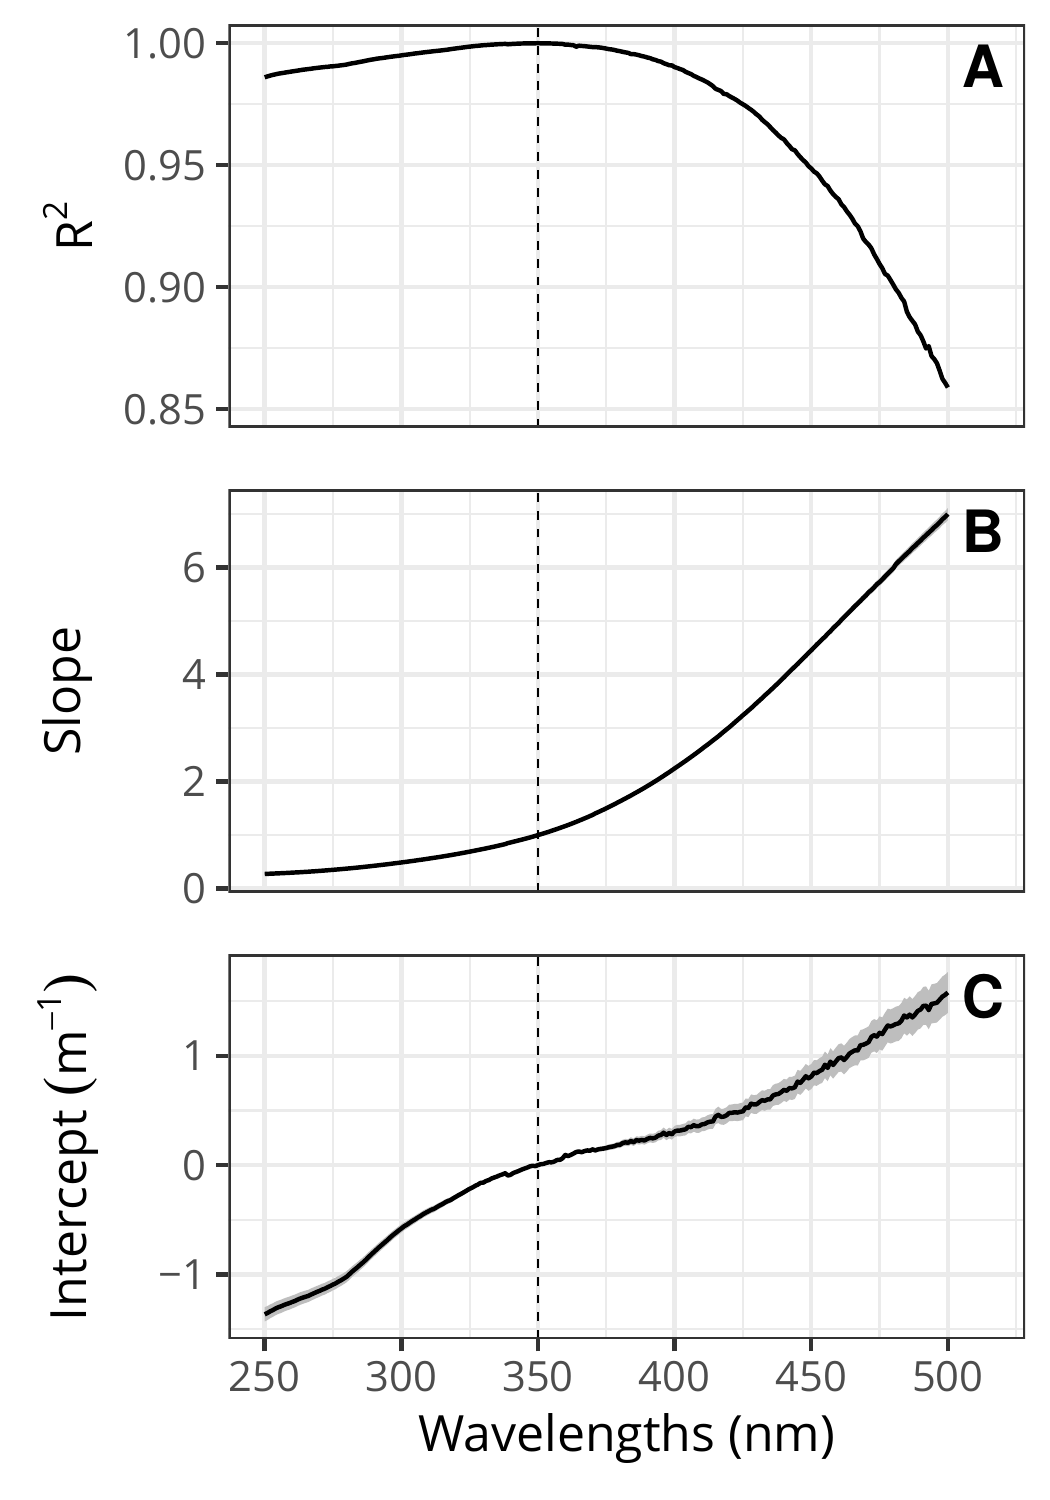
\includegraphics[scale = 1]{../../graphs/fig2}
	\caption{Results of the linear regressions between $a_{CDOM}(350)$ and $a_{CDOM}(\lambda)$. (A) Determination coefficient ($R^2$), (B) slope and (C) intercept of the linear regressions. Panels contain the results of 251 linear models, each based on 2190 data points. Note that at $\lambda = 350$ nm, $R^2 = 1$, slope = 1 and intercept = 0.}
\end{figure}

\clearpage
\newpage

\begin{figure}[h]
	\centering
	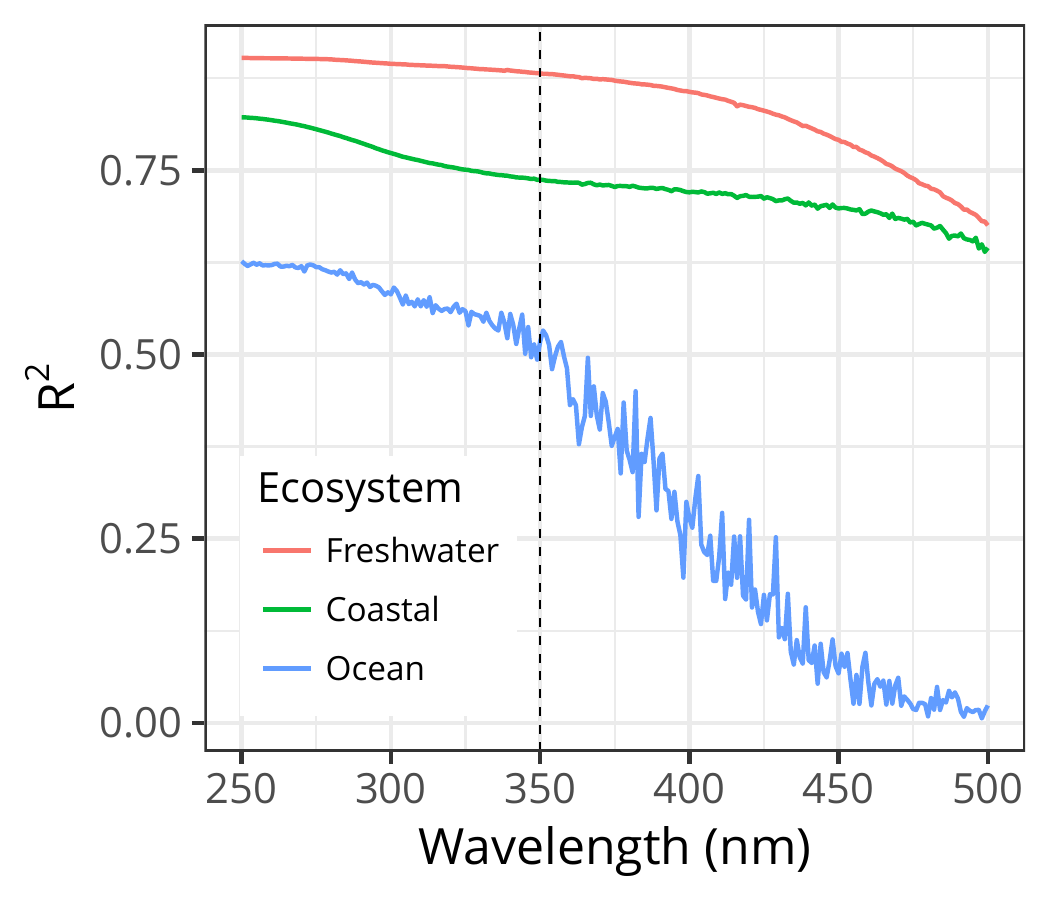
\includegraphics[scale = 0.75]{../../graphs/fig3}
	\caption{Boxplots showing the distribution of (A) absorption coefficients at 350 nm ($a_{CDOM}(350)$), (B) dissolved organic carbon (DOC) and (C) the \textit{so-called} $a^*$. Y-axis are log-transformed given the wide ranges spanned by the data.}
\end{figure}

\begin{figure}[h]
	\centering
	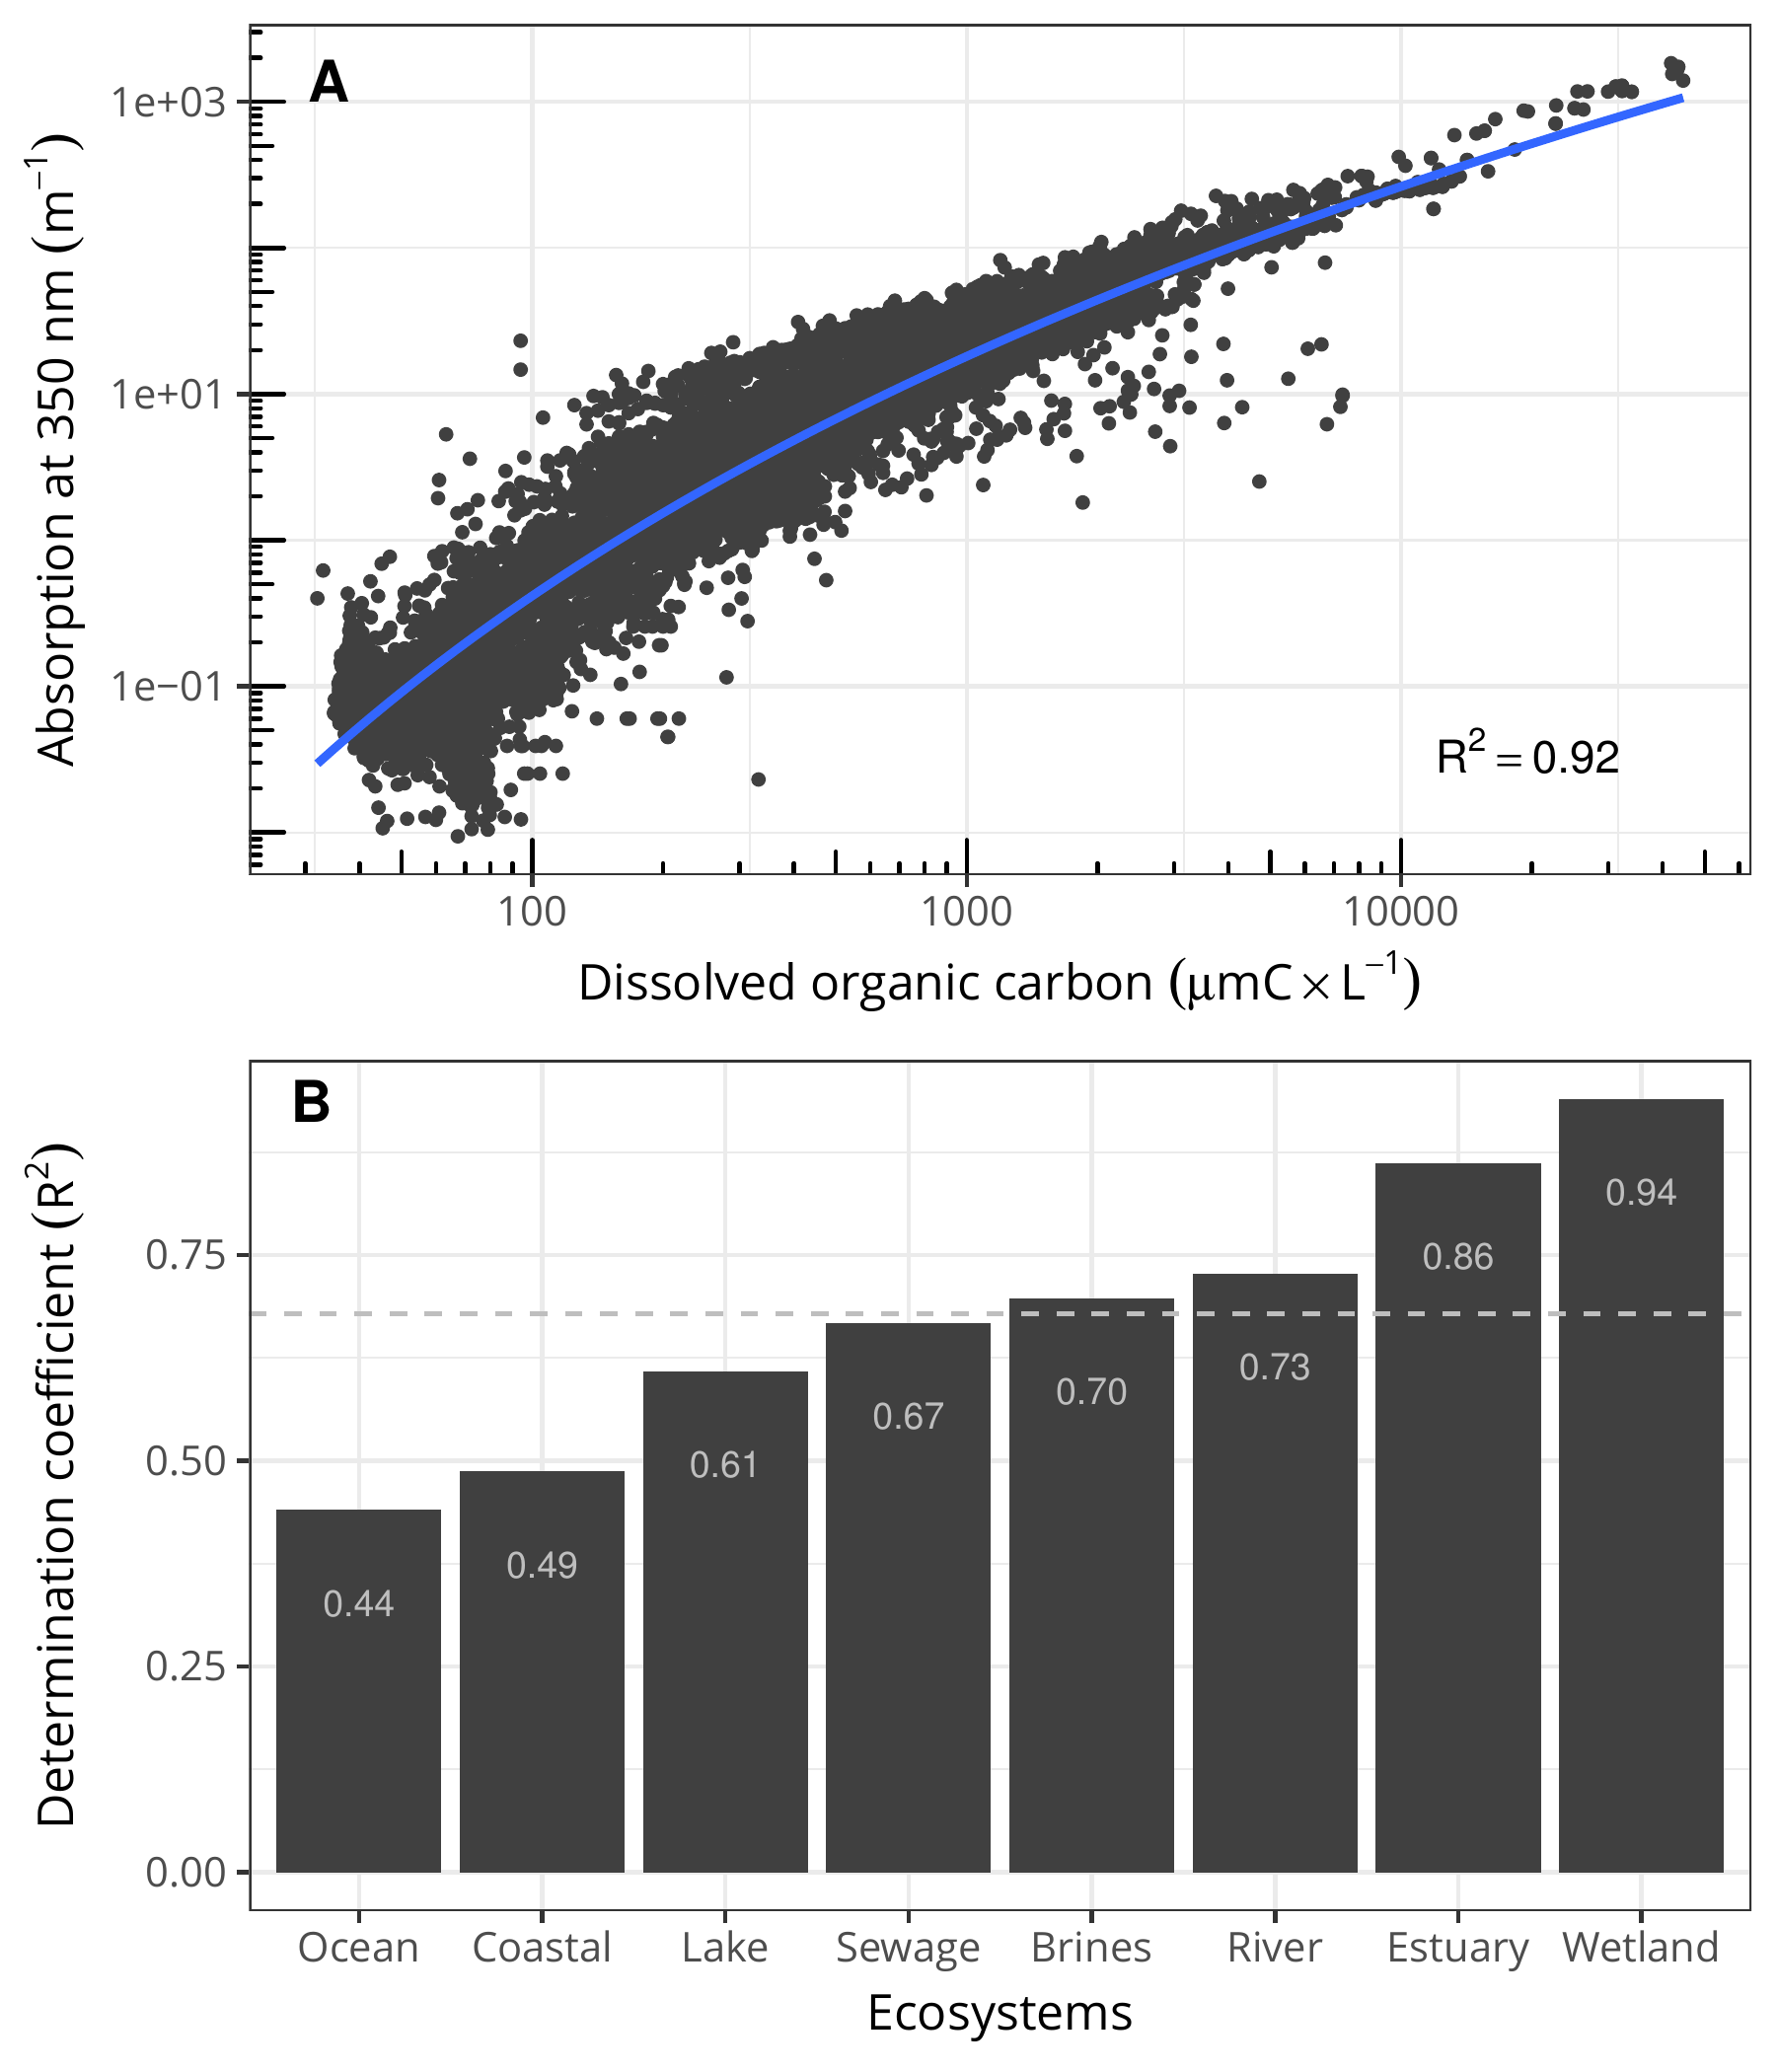
\includegraphics[scale = 1]{../../graphs/fig5}
	\caption{Global relationship between absorption at 350 nm $a_{CDOM}(350)$ and dissolved organic carbon ($n = 11431$). The blue line is the fitted values of a linear model $y = log(x)$.}
\end{figure}


\end{document}
